\documentclass[12pt]{beamer}
\newenvironment{ConCodigo}[1]
  {\begin{frame}[fragile,environment=ConCodigo]{#1}}
  {\end{frame}}
\graphicspath{{Imagenes/}{../Imagenes/}}
\usepackage[utf8]{inputenc}
\usepackage[spanish]{babel}
\usepackage{hyperref}
\usepackage{etex}
\reserveinserts{28}
\usepackage{amsmath}
\usepackage{amsthm}
\usepackage{mathtools}
\usepackage{multicol}
\usepackage{multirow}
\usepackage{tabulary}
%\usepackage{tabularx}
\usepackage{booktabs}
\usepackage{nccmath}
\usepackage{biblatex}
\usepackage{epstopdf}
\usepackage{graphicx}
\usepackage{siunitx}
\sisetup{scientific-notation=true}
%\usepackage{fontspec}
\usepackage{lmodern}
\usepackage{float}
\usepackage[format=hang, font=footnotesize, labelformat=parens]{caption}
\usepackage[autostyle,spanish=mexican]{csquotes}
\usepackage{standalone}
\usepackage{tikz}
\usepackage[siunitx]{circuitikz}
\usetikzlibrary{arrows,patterns,shapes}
\usetikzlibrary{decorations.markings}
\usetikzlibrary{arrows}
\usepackage{color}
%\usepackage{beton}
%\usepackage{euler}
%\usepackage[T1]{fontenc}
\usepackage[sfdefault]{roboto}  %% Option 'sfdefault' only if the base font of the document is to be sans serif
\usepackage[T1]{fontenc}
\renewcommand*\familydefault{\sfdefault}
\DeclareGraphicsExtensions{.pdf,.png,.jpg}
\usepackage{hyperref}
\renewcommand {\arraystretch}{1.5}
\newcommand{\python}{\texttt{python}}
\usefonttheme[onlymath]{serif}
\setbeamertemplate{navigation symbols}{}
\usetikzlibrary{patterns}
\usetikzlibrary{decorations.markings}
\tikzstyle{every picture}+=[remember picture,baseline]
%\tikzstyle{every node}+=[inner sep=0pt,anchor=base,
%minimum width=2.2cm,align=center,text depth=.15ex,outer sep=1.5pt]
%\tikzstyle{every path}+=[thick, rounded corners]
\setbeamertemplate{caption}[numbered]
\newcommand{\ptm}{\fontfamily{ptm}\selectfont}
%Se usa la plantilla Warsaw modificada con spruce
\mode<presentation>
{
  \usetheme{Warsaw}
  \setbeamertemplate{headline}{}
  \useoutertheme{default}
  \usecolortheme{beaver}
  \setbeamercovered{invisible}
}
\AtBeginSection[]
{
\begin{frame}<beamer>{Contenido}
\normalfont\mdseries
\tableofcontents[currentsection]
\end{frame}
}

\usepackage{listings}
\lstset{ %
language=Python,                % choose the language of the code
basicstyle=\small,       % the size of the fonts that are used for the code
numbers=left,                   % where to put the line-numbers
numberstyle=\small,      % the size of the fonts that are used for the line-numbers
stepnumber=1,                   % the step between two line-numbers. If it is 1 each line will be numbered
numbersep=5pt,                  % how far the line-numbers are from the code
backgroundcolor=\color{white},  % choose the background color. You must add \usepackage{color}
showspaces=false,               % show spaces adding particular underscores
showstringspaces=false,         % underline spaces within strings
showtabs=false,                 % show tabs within strings adding particular underscores
frame=single,   		% adds a frame around the code
tabsize=2,  		% sets default tabsize to 2 spaces
captionpos=b,   		% sets the caption-position to bottom
breaklines=true,    	% sets automatic line breaking
breakatwhitespace=false,    % sets if automatic breaks should only happen at whitespace
escapeinside={\%},          % if you want to add a comment within your code
stringstyle =\color{magenta},
keywordstyle = \color{blue},
commentstyle = \color{green},
identifierstyle = \color{red}
}
\title{EDO con valores en las frontera}
\subtitle{Ecuaciones diferenciales ordinarias 4}
%\subtitle{Curso de Física Computacional}
\author[]{M. en C. Gustavo Contreras Mayén}
\begin{document}
\maketitle
\fontsize{14}{14}\selectfont
\spanishdecimal{.}
\begin{frame}{Contenido}
\tableofcontents[pausesections]
\end{frame}
\section{Problemas con valores en la frontera y valores propios.}
\begin{frame}
\frametitle{Problemas con valores en la frontera y valores propios}
Otra tipo de problemas de la física requiere la solución de ecuaciones diferenciales con valores de las magnitudes físicas o sus derivadas en las fronteras de una región.
\\
\medskip
\pause
Por ejemplo:
\begin{itemize}
\item La solución de la ecuación de Poisson con una  distribución de carga dada y valores conocidos de potencial electrostático en la frontera.
\item La ecuación de Schrödinger estacionaria con un potencial dado y  
condiciones de frontera.
\end{itemize}
\end{frame}
\begin{frame}
Un problema de típico de valores en la frontera en física, por lo general se presenta en forma de una ecuación diferencial de segundo orden:
\begin{equation}
u'' = f(u, u';x)
\label{eq:ecuacion1}
\end{equation} 
donde $u$ es una función de $x$; $u'$ y $u''$ son las derivadas de primer y segundo orden de $u$ con respecto a $x$, $f(u,u';x)$ es una función de $u$, $u'$ y $x$. Tanto $u$ o $u'$ están dadas como puntos en la frontera.
\end{frame}
\begin{frame}
Considera que sin pérdida de generalidad, siempre podemos elegir un sistema coordenado tal que las fronteras del sistema sean $x=0$ y $x=1$, siempre y cuando el sistema sea finito.
\\
\medskip
Por ejemplo, para un problema dado si el sistema tiene las fronteras en $x=x_{1}$ y $x=x_{2}$, siempre podemos hacer $x'=0$ y $x'=1$ con una transformación
\begin{equation}
x' = \dfrac{x-x_{1}}{x_{2} - x_{1}}
\end{equation} 
\end{frame}
\begin{frame}
Para problemas de una dimensión, tenemos un total de cuatro tipo de condiciones de frontera:
\begin{enumerate}
\item $u(0) = u_{0}$ y $u(1) = u_{1}$ 
\item $u(0) = u_{0}$ y $u'(1) = v_{1}$
\item $u'(0) = v_{0}$ y $u(1) = u_{1}$
\item $u'(0) = v_{0}$ y $u'(1) = v_{1}$   
\end{enumerate}
\end{frame}
\begin{frame}
Un problema de valores en la frontera es más difícil de resolver que un problema de valores iniciales.
\\
\medskip
Si queremos resolver un problema de valores iniciales del tipo de la ecuación (\ref{eq:ecuacion1}), donde re-emplazamos $x$ por $t$ y las condiciones iniciales $u(0) = u_{0}$ y $u'(0) = v_{0}$, podemos transformar la ED en un conjunto de dos EDO-1, como lo hemos venido haciendo.
\\
\medskip
Sin embargo, para el problema de valores en la frontera (VEF), sólo conocemos $u(0)$ o $u'(0)$, que no es lo suficiente para utilizar alguno de los algoritmos que conocemos para las EDO-1 de valores iniciales (Taylor, Euler, RK4)
\end{frame}
\section{Problemas de valores propios}
\begin{frame}
\frametitle{Problemas de valores propios}
Los problemas típicos de valores propios son aún más complicados, ya que al menos un parámetro más, el \emph{valor propio}, está involucrado en la ecuación, por ejemplo:
\begin{equation}
u'' = f(u, u'; x; \lambda)
\label{eq:ecuacion_vp}
\end{equation}
junto con un conjunto de condiciones de frontera, definen un problema de valores propios.
\\
\medskip
El valor propio $\lambda$(también llamado \emph{eigenvalor}), puede tener sólo algunos valores determinados  con el fin de proporcionar soluciones aceptables de la ecuación, con las condiciones de frontera establecidas.
\end{frame}
\begin{frame}
\frametitle{Ejemplo}
Consideremos las vibraciones longitudinales a lo largo de una cuerda elástica, la ecuación que describe la solución estacionaria de las ondas elásticas es
\begin{equation}
u''(x) = - k^{2} u(x)
\end{equation}
donde $u(x)$ es el desplazamiento sobre el punto de equilibrio $x$ y los valores permitidos de $k^{2}$ son los valores propios del problema.
\\
\medskip
El vector de onda $k$ en la ecuación, está relacionado con la velocidad de fase $c$ de la onda a lo largo de la cuerda, y la frecuencia angular $\omega$ permitida, por la relación
\begin{equation}
\omega = ck
\end{equation}
\end{frame}
\begin{frame}
Si los extremos de la cuerda están fijos ($x=0$ y $x=1$), las condiciones de frontera son por tanto: $u(0)=u(1)=0$. Si un extremo de la cuerda ($x=0$) está fijo y el otro libre ($x=1$), las condiciones de frontera ahora son $u(0)=0$ y $u'(0)=1$. Para este problema, podemos obtener una solución analítica.
\\
\medskip
Por ejemplo, si los extremos de la cuerda están fijos, las funciones propias
\begin{equation}
u_{l}(x) = \sqrt{2} \sin k_{l} x
\end{equation}
son las posibles soluciones de la ED.
\\
\medskip
\pause
Los valores propios están dados por
\begin{equation}
k_{l}^{2} = (l \pi)^{2}
\end{equation}
con $l=1,2,\ldots,\infty$. 
\end{frame}
\begin{frame}
La solución completa de las ondas a lo largo de la cuerda elástica están dadas por una combinación lineal de las funciones propias con las soluciones de valores iniciales, en este caso
\begin{equation}
u(x,t) = \sum_{l=1}^{\infty} (a_{l} \sin \omega_{l} t + b_{i} \cos \omega_{l} t) u_{l}(x)
\end{equation}
donde $\omega_{l} = c k_{l}$, $a_{l}$ y $b_{l}$ son los coeficientes determinados por las condiciones iniciales.
\end{frame}
\section{Método de disparo}
\begin{frame}
\frametitle{Método de disparo}
Un método sencillo para resolver problemas de ED-CVF (ecuación \ref{eq:ecuacion1}) y los problemas de valores propios (ecuación \ref{eq:ecuacion_vp}), es el llamado \emph{método de disparo}.
\\
\medskip
Veamos cómo funciona para problemas CVF y luego, generalizar para problemas de valores propios.
\end{frame}
\begin{frame}
Como hemos hecho en el caso de tener un problema de una ED de orden 2, hacemos un cambio de variable, para dejar un sistema de EDO-1, haciendo $y_{1}=u$ y $y_{2}=u'$, por tanto
\begin{eqnarray}
\dfrac{dy_{1}}{dx} &=& y_{2} \\
\dfrac{dy_{2}}{dx} &=& f(y_{1}, y_{2}; x)
\end{eqnarray}
suponiendo las siguientes CVF $u(0)= u_{0}$ y $u(1)= u_{1}$. Para otro tipo de problemas con otras CVF, se pueden resolver de manera similar.
\end{frame}
\begin{frame}
El punto importante es hacer que el problema se parezca a un problema de valores iniciales, utilizando un parámetro que se ajuste, por lo que la solución se obtiene al variar el parámetro.
\\
\medskip
Como $u(0)$ ya está dado, podemos hacer una estimación para la derivada de primer orden en $x=0$, por ejemplo, $u'(0)=\alpha$. Donde $\alpha$ es el parámetro que estará variando.
\\
\medskip
\pause
Para un valor específico de $\alpha$, podemos integrar la ecuación para $x=1$ con alguna de las técnicas que hemos visto para EDO-1.
\end{frame}
\begin{frame}
Considerando que la elección inicial de  $\alpha$ difícilmente pudiese ser la derivada en $x = 0$, el valor de la función $u_{\alpha} (1)$, resultante de la integración con $u'(0) = \alpha$  para $x = 1$, podría no ser el mismo que $u_{1}$.
\\
\medskip
La idea del método de disparo es utilizar alguno de los algoritmos de búsqueda de la raíz para encontrar la $\alpha$ apropiada, que asegure $f(\alpha) = u_{\alpha} (1) - u_{1} = 0$, con una tolerancia $\delta$ dada.
\end{frame}
\begin{frame}
\frametitle{Ejemplo}
Hagamos un ejercicio para revisar el método. Sea la siguiente EDO-2
\begin{equation}
u'' = - \dfrac{\pi^{2}}{4}(u+1)
\end{equation}
y las CVF son $u(0)=0$ y $u(1)=1$. 
\\
\medskip
\pause
Definimos $y_{1}=u$ y $y_{2}=u'$, por lo que tenemos ahora
\begin{eqnarray}
\dfrac{dy_{1}}{dx} &=& y_{2} \\
\dfrac{dy_{2}}{dx} &=& - \dfrac{\pi^{2}}{4}(y_{1} + 1)
\end{eqnarray}
\end{frame}
\begin{frame}
Asumimos que la ecuación tiene los valores iniciales $y_{1}(0)=0$ y $y_{2}(0) = \alpha$.
\\
\medskip
\pause
El valor de $\alpha$ tendrá que ajustarse para que $f(\alpha) = u_{\alpha}(1) - 1 = 0$.
\\
\medskip
Podemos combinar el método de la secante y resolver el sistema de EDO-1 como lo hemos venido haciendo
\end{frame}
\begin{frame}[fragile]
\frametitle{Solución con $y0 = array([0.0,\alpha=1.0])$}
\begin{figure}
	\centering
	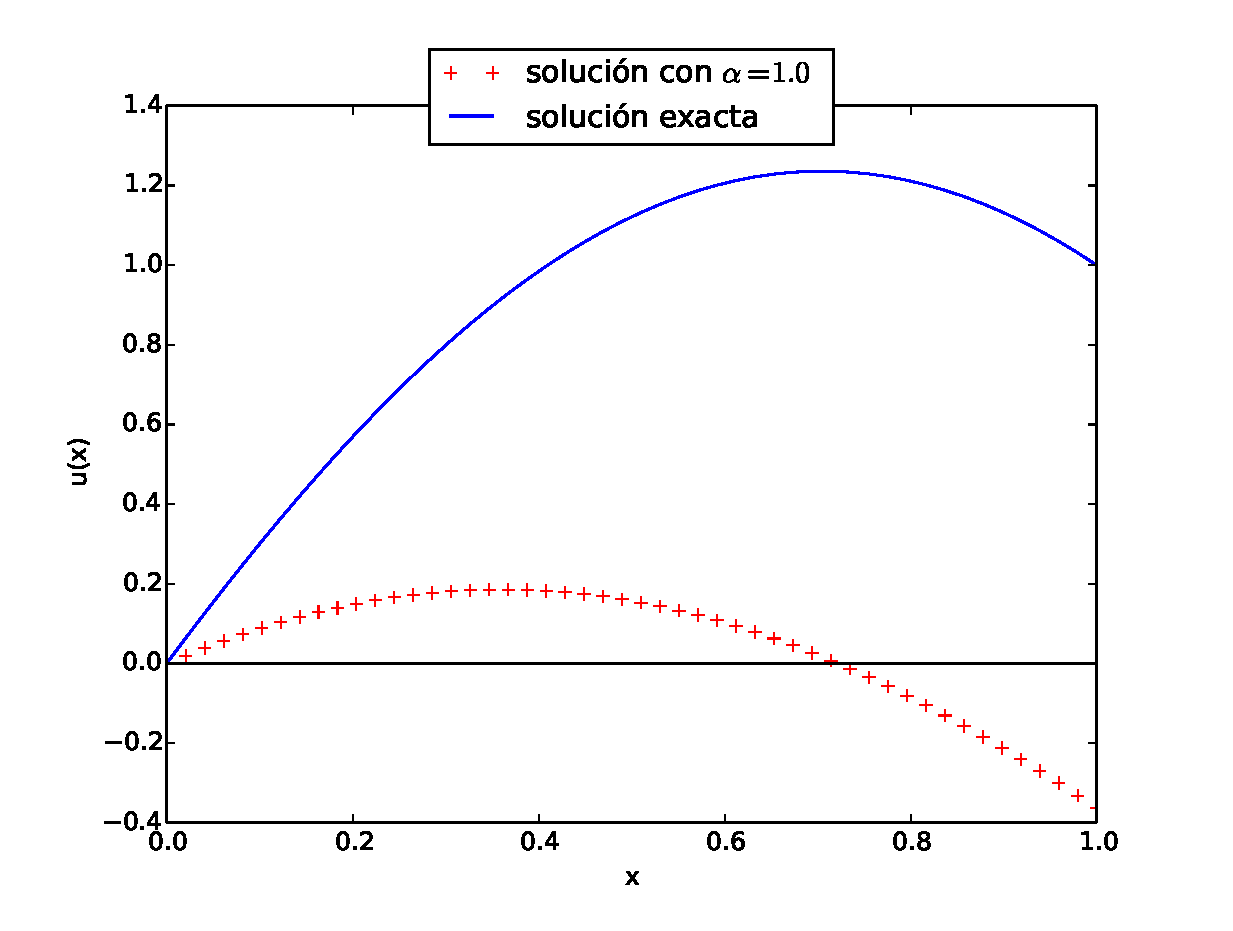
\includegraphics[scale=0.5]{MetodoDisparo2014_01.eps}
\end{figure}
\end{frame}
\begin{frame}[fragile]
\frametitle{Solución con $y0 = array([0.0,\alpha=4.0])$}
\begin{figure}
	\centering
	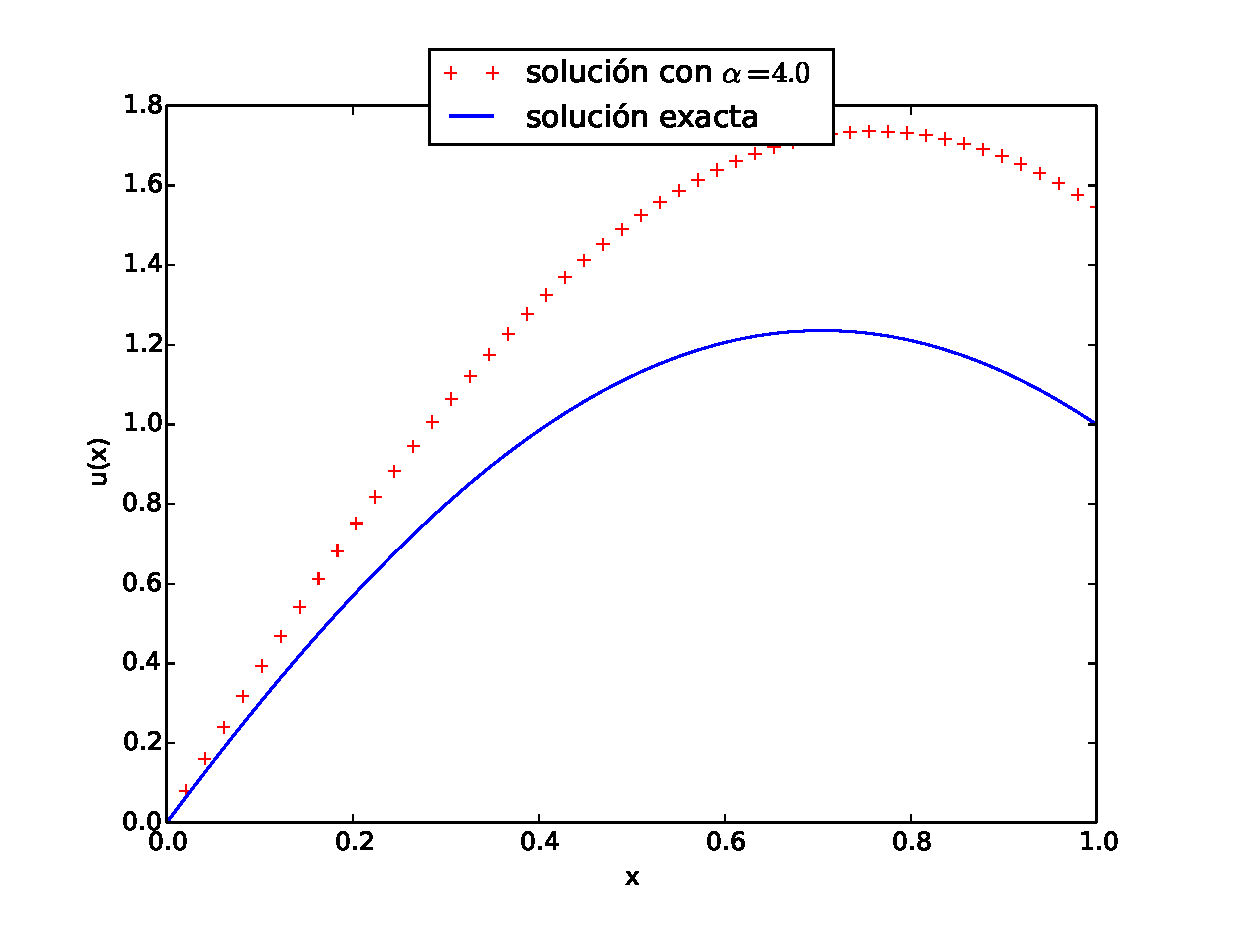
\includegraphics[scale=0.5]{MetodoDisparo2014_02.eps}
\end{figure}
\end{frame}
\begin{frame}
\frametitle{¿Qué hacemos?}
El siguiente paso es encontrar el valor de la raíz en donde $f(\alpha) = u_{\alpha}(1) - 1 = 0$.
\\
\medskip

Revisando los valores que obtenemos para $\alpha$:
\\
\medskip
$u_{1.0}(1) = -0.3633$ \\
$u_{4.0}(1) = 1.5464$
\\
\medskip
Por lo que necesariamente hay una raíz que debemos de utilizar para sustituirla en nuestro problema.
\end{frame}
\begin{frame}
El problema CVF se resuelve de manera exacta, la solución analítica es:
\begin{equation}
u(x) = \cos\left(\frac{x \pi}{2}\right) + 2 \sin \left(\frac{x \pi}{2}\right) -1
\end{equation}
\end{frame}
\begin{frame}
\frametitle{Pasos a realizar}
\begin{enumerate}
\item Construir una tabla de valores $\alpha$ y $f(\alpha) = u_{\alpha}(1) - 1$.
\item Usando el método de la secante, obtener el valor de la raíz tal que $f(\alpha)=0$. El método de la secante que construimos en el Tema 2, requiere de dos valores iniciales, para esa función, dabamos una función $f$ que python evalúa al momento, ahora nuestra función es una tabla de pares ordenados $\alpha$ y $f(\alpha)$, por lo que hay que ajustar nuestro código para que reciba esos valores y nos devuelva la raíz.
\item El valor de la raíz, lo usamos como argumento en $y0=[0.0, \alpha]$ y resolvemos la ecuación diferencial.
\end{enumerate}
\end{frame}
\begin{frame}[fragile]
\frametitle{Solución con $y0 = array([0.0,\alpha=??])$}
\begin{figure}
	\centering
	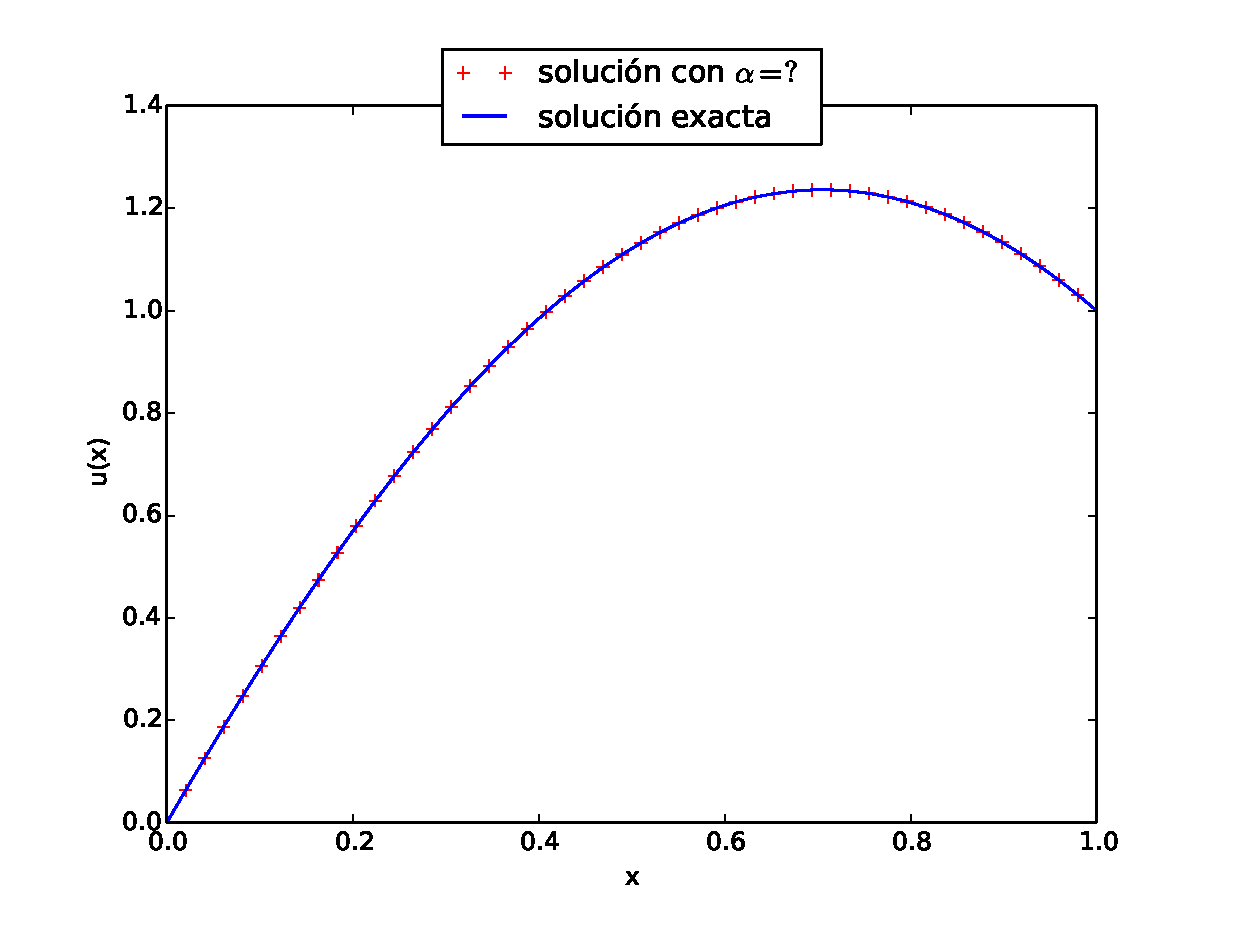
\includegraphics[scale=0.5]{MetodoDisparo2014_03.eps}
\end{figure}
\end{frame}
\begin{frame}
Problemas con otros tipos de CVF se pueden resolver de manera similar. Por ejemplo:
\\
\medskip
si $u'(0)=v_{0}$ y $u(1)=u_{1}$ están dados, podemos hacer una estimación de $u(0)=\alpha$ e integrar el conjunto de ecuaciones de $y_{1}$ y $y_{2}$ en $x=1$. La raíz a buscar está en $f(\alpha) = u_{\alpha}(1) - u_{1} = 0$. Aquí el valor de $u_{\alpha}(1)$ es el resultado de la ecuación con $u(0)=\alpha$.
\end{frame}
\begin{frame}
Cuando se aplica el método de disparo para los problemas de valores propios, el parámetro a ajustar no es mayor que el valor propio del problema.
\\
\medskip
Por ejemplo, si están dados $u(0)=u_{0}$ y $u(1)=u_{1}$, podemos integrar la ecuación con $u'(0)= \alpha$, que es un valor pequeño. Luego, buscamos la raíz de $f(\lambda) = u_{\lambda}(1) - u_{1}=0$ variando $\lambda$.
\\
\medskip
Cuando $f(\lambda)=0$ se satisface, obtenemos un valor propio aproximado $\lambda$ y el correspondiente estado propio de la solución normalizada de $u_{\lambda}(x)$.
\end{frame}
\section{Ecuaciones lineales y problemas tipo Sturm-Liouville}
\begin{frame}
\frametitle{Ecuaciones lineales y problemas tipo Sturm-Liouville}
Muchos problemas de valores propios y VCF se expresan como una ecuación lineal
\begin{equation}
u'' = d(x) u' + q(x) u = s(x)
\end{equation}
donde $d(x)$, $q(x)$ y $s(x)$ son funciones de $x$.
\\
\medskip
Suponemos que las condiciones de frontera son $u(0)=u_{0}$ y $u(1)=u_{1}$.
\end{frame}
\begin{frame}
Si las funciones $d(x)$, $q(x)$ y $s(x)$ son ''bien portadas'', es decir, \emph{suaves}, podemos resolver la ecuación anterior usando el método de disparo que ya revisamos.
\\
\medskip
Se puede demostrar que no se necesita  hacer una búsqueda extendida del parámetro $\alpha$, para obtener $f(\alpha) = u_{\alpha}(1) - u_{1} = 0$, ya que por el principio de superposición de ecuaciones lineales: cualquier combinación lineal de la solución, es también solución de la ecuación.
\\
\medskip
Por lo tanto, requerimos de dos soluciones $u_{\alpha_{0}}(x)$ y $u_{\alpha_{1}}(x)$, donde $\alpha_{0}$ y $\alpha_{1}$ son dos parámetros diferentes.
\end{frame}
\begin{frame}
La solución de la ecuación está dada por:
\begin{equation}
u(x) = a u_{\alpha_{0}}(x) + b u_{\alpha_{1}}(x)
\end{equation}
donde $a$ y $b$ están dadas por $u(0)= u_{0}$ y $u(1) = u_{1}$. Nótese que $u_{\alpha_{0}}(0)=u_{\alpha_{1}}(0) = u(0) = u_{0}$, por lo que tenemos
\begin{eqnarray}
a + b &=& 1 \\
u_{\alpha_{0}}(1) a + u_{\alpha_{1}} (1) b &=& u_{1}
\end{eqnarray}
\end{frame}
\begin{frame}
Lo que nos lleva a
\begin{eqnarray}
a &=& \dfrac{u_{\alpha_{1}} (1) - u_{1}}{u_{\alpha_{1}} (1)-u_{\alpha_{0}} (1)} \\
b &=& \dfrac{ u_{1}- u_{\alpha_{0}} (1)}{u_{\alpha_{1}} (1)-u_{\alpha_{0}} (1)}
\end{eqnarray}
\end{frame}
\begin{frame}
\frametitle{Ejercicio para el examen}
Usando el esquema indicado, resuelve el mismo problema:
\begin{equation}
u'' = - \dfrac{\pi^{2}}{4}(u+1)
\end{equation}
y las CVF son $u(0)=0$ y $u(1)=1$. 
\\
\bigskip
El resultado debe de ser consistente con la primera solución.
\end{frame}
\begin{frame}
Un tipo de ecuaciones lineales importantes en la física, son los llamados problemas tipo \emph{Sturm-Liouville}, definidos por
\begin{equation}
[p(x) u'(x)]' + q(x) u(x) = s(x)
\end{equation}
donde vemos una combinación de términos con primeras y segundas derivadas. Las funciones $p(x)$, $q(x)$ y $s(x)$ son los coeficientes de $x$.
\\
\medskip
Para la mayoría de los problemas se tiene que $s(x)=0$ y $q(x) = - r(x) +  \lambda w(x)$, donde $\lambda$ es el valor propio de la ecuación, $r(x)$ y $w(x)$ son coeficientes redefinidos de la función.
\end{frame}
\end{document}